\documentclass[a4paper, oneside]{article}
\usepackage[margin=0.125in]{geometry}
\usepackage{calc}
\usepackage[skip=0pt]{parskip}

\usepackage[dvipsnames]{xcolor}
\usepackage{tikz}
\usepackage{booktabs}
\usepackage{fontspec}
\usepackage{multirow}
\usepackage{contour}
\contournumber{256}
\contourlength{0.1cm}

\definecolor{wolfblue}{HTML}{0038A8}
\definecolor{dragongreen}{HTML}{008000}
\definecolor{eaglered}{HTML}{A52A2A}

\colorlet{Character}{Brown}
\colorlet{Intrigue}{wolfblue}
\colorlet{Ritual}{dragongreen}

\tikzset{wolf/.pic={
\node () at (0,0) {
\includegraphics[scale=1.33]{Images/wolf_gray.png}};
}}

\tikzset{eagle/.pic={
\node () at (0,0) {
\includegraphics[scale=1.33]{Images/eagle_brown.png}};
}}

\tikzset{seahorse/.pic={
\node () at (0,0) {
\includegraphics[scale=3.1]{Images/seahorse.png}};
}}

\tikzset{hydra/.pic={
\node () at (0,0) {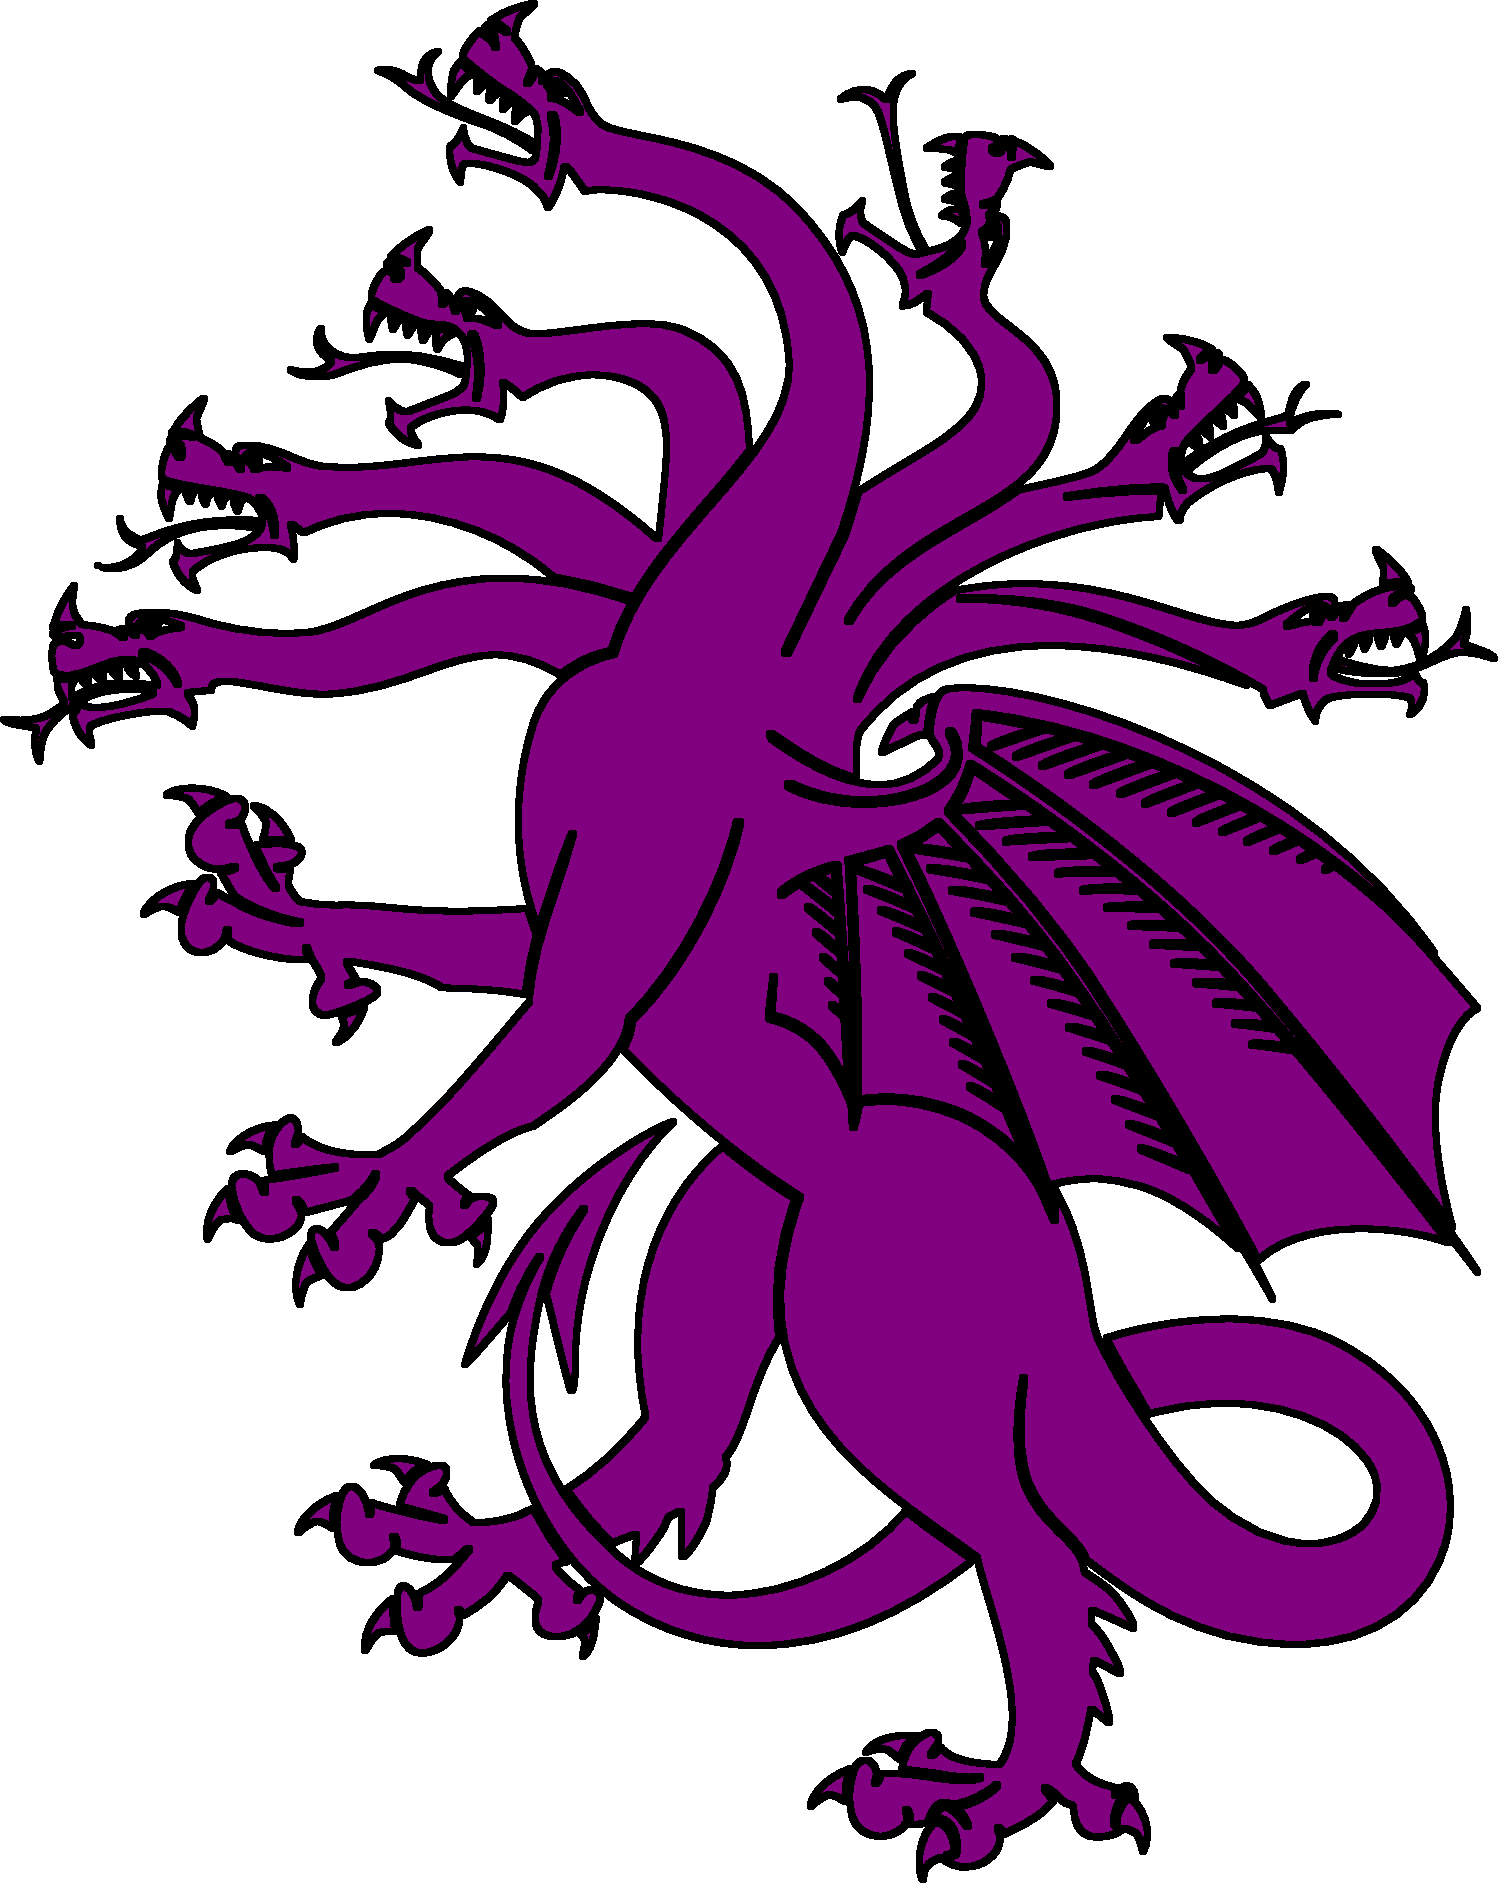
\includegraphics[scale=2.0]{Images/hydra.png}};
}}

\usepackage[dvipsnames]{xcolor}
\usepackage{tikz}
\usepackage{calc}
\usepackage{fontspec}
\setmainfont[Scale=3.0]{Cinzel}

\definecolor{paper}{HTML}{F1EBDB}
\definecolor{wolfblue}{HTML}{0038A8}
\definecolor{dragongreen}{HTML}{008000}
\definecolor{eaglered}{HTML}{A52A2A}
\definecolor{kidagold}{HTML}{FFD700}
\definecolor{flatgray}{HTML}{5F6467}

\newlength\myrblen
\newlength\myrbht
\newlength\myrbarc
\setlength\myrblen{1cm}
\setlength\myrbht{1.1cm}
\setlength\myrbarc{0.1cm}

\tikzset{ribbon/.pic={%
\path
  (0,0) --
  ++(3\myrblen,0) to[out=0,in=0,looseness=3] coordinate[midway] (aux1)
  ++(0,-\myrbarc) --
  ++(-\myrblen,0) to[out=180,in=180,looseness=3] coordinate[midway] (aux2)
  ++(0,- \myrbarc) --
  ++(5\myrblen,0) to[out=0,in=0,looseness=3] coordinate[midway] (aux3)
  ++(0, \myrbarc) --
  ++(-\myrblen,0) to[out=180,in=180,looseness=3] coordinate[midway] (aux4)
  ++(0, \myrbarc) --
  ++(3\myrblen,0) --
  ++(-0.5\myrbht,-0.5\myrbht) --
  ++(0.5\myrbht,-0.5\myrbht) --
  ++(-9\myrblen,0) --
  ++(0.5\myrbht,0.5\myrbht) --
  ++(-0.5\myrbht,0.5\myrbht) --
    cycle;
\draw[thick, fill=paper!75!black]
  (aux1) -- ++(0,-0.5\myrbht) coordinate (aux7) -- (aux2|-aux7) -- (aux2|-aux1) -- cycle;  
\draw[thick, fill=paper!75!black]
  (aux4) -- ++(0,-0.5\myrbht) coordinate (aux8) -- (aux3|-aux8) -- (aux3|-aux4) -- cycle;  
\draw[thick,fill=paper]
  (0,0) --
  ++(3\myrblen,0) to[out=0,in=0,looseness=3] coordinate[midway] (aux1)
  ++(0,-\myrbarc) --
  ++(-\myrblen,0) to[out=180,in=180,looseness=3] coordinate[midway] (aux2)
  ++(0,- \myrbarc) --
  ++(5\myrblen,0) to[out=0,in=0,looseness=3] coordinate[midway] (aux3)
  ++(0, \myrbarc) --
  ++(-\myrblen,0) to[out=180,in=180,looseness=3] coordinate[midway] (aux4)
  ++(0, \myrbarc) --
  ++(3\myrblen,0) --
  ++(-0.5\myrbht,-0.5\myrbht) --
  ++(0.5\myrbht,-0.5\myrbht) --
  ++(-9\myrblen,0) --
  ++(0.5\myrbht,0.5\myrbht) --
  ++(-0.5\myrbht,0.5\myrbht) --
   cycle;
\path
  (aux2) {[rounded corners=1.5pt] -- 
  ++(0,\dimexpr-\myrbht-1.5\myrbarc\relax) coordinate (aux5) -- 
  (aux3|-aux5)} -- 
  (aux3);
\fill[paper]
  ([yshift=-\myrbarc]aux2) {[rounded corners=1.5pt] -- 
  ++(0,\dimexpr-\myrbht-0.5\myrbarc\relax) -- 
  (aux3|-aux5)} -- 
  ([yshift=-\myrbarc]aux3);
\draw[thick]
  (aux2) {[rounded corners=1.5pt] -- 
  ++(0,\dimexpr-\myrbht-1.5\myrbarc\relax) coordinate (aux5) --  
  (aux3|-aux5)} -- 
  (aux3);
  
\node[inner sep=0pt] () at (4.5\myrblen, -2.5\myrbarc - 0.5\myrbht) {#1};
}}

\tikzset{shield/.pic={
	\draw[ultra thick] (0, 0cm) -- (0, 3cm) -- (9cm, 3cm) -- (9cm, 0cm) arc (0:-60:9cm) arc (240:180:9cm);
}}

\tikzset{Sorrell/.pic={
	\begin{scope}
	\clip (0,0cm) -- (0,3cm) -- (9cm,3cm) -- (9cm,0cm) arc (0:-60:9cm) arc (240:180:9cm);
	
	\draw[thick, fill=eaglered] (0, -2cm) -- (4.5cm, -2cm) -- (4.5cm, 3cm) -- (0, 3cm) -- cycle;
	\draw[thick, fill=white] (9cm, -2cm) -- (4.5cm,-2cm) -- (4.5cm, 3cm) -- (9cm,3cm) -- cycle;
	\draw[thick, fill=white] (0,-2cm) -- (4.5cm, -2cm) -- (4.5cm, -9) -- (0,-9cm) -- cycle;
	\draw[thick, fill=eaglered] (9cm, -2cm) -- (4.5cm, -2cm) -- (4.5cm, -9cm) -- (9cm,-9cm) -- cycle;

\end{scope}
}}

\tikzset{Marus/.pic={
\begin{scope}
	\clip (0,0cm) -- (0,3cm) -- (9cm,3cm) -- (9cm,0cm) arc (0:-60:9cm) arc (240:180:9cm);

	\fill[wolfblue] (0,0cm) -- (0,3cm) -- (9cm,3cm) -- (9cm,0cm) arc (0:-60:9cm) arc (240:180:9cm);
	\draw[thick, fill=White] (0, 1cm) -- (0, 3cm) -- (2cm, 3cm) -- (14cm, -9cm) -- (14cm, -11cm) -- (12cm, -11cm) -- cycle;

\end{scope}
}}

\tikzset{Kida/.pic={
\begin{scope}
	\clip (0,0cm) -- (0,3cm) -- (9cm,3cm) -- (9cm,0cm) arc (0:-60:9cm) arc (240:180:9cm);
	
	\fill[kidagold] (0,0cm) -- (0,3cm) -- (9cm,3cm) -- (9cm,0cm) arc (0:-60:9cm) arc (240:180:9cm);
	\draw[ultra thick, fill=black] (2cm, 3cm) -- (7cm, 3cm) -- (4.5cm, -8cm) -- cycle;

\end{scope}
}}

\tikzset{Argent/.pic={
\begin{scope}
	\clip (0,0cm) -- (0,3cm) -- (9cm,3cm) -- (9cm,0cm) arc (0:-60:9cm) arc (240:180:9cm);
	
	\fill[White] (0,0cm) -- (0,3cm) -- (9cm,3cm) -- (9cm,0cm) arc (0:-60:9cm) arc (240:180:9cm);
\end{scope}
}}

\tikzset{Hydra/.pic={
\begin{scope}
	\clip (0,0cm) -- (0,3cm) -- (9cm,3cm) -- (9cm,0cm) arc (0:-60:9cm) arc (240:180:9cm);
	
	\fill[White] (0,0cm) -- (0,3cm) -- (9cm,3cm) -- (9cm,0cm) arc (0:-60:9cm) arc (240:180:9cm);
	\node () at (4.5cm, -1.5cm) {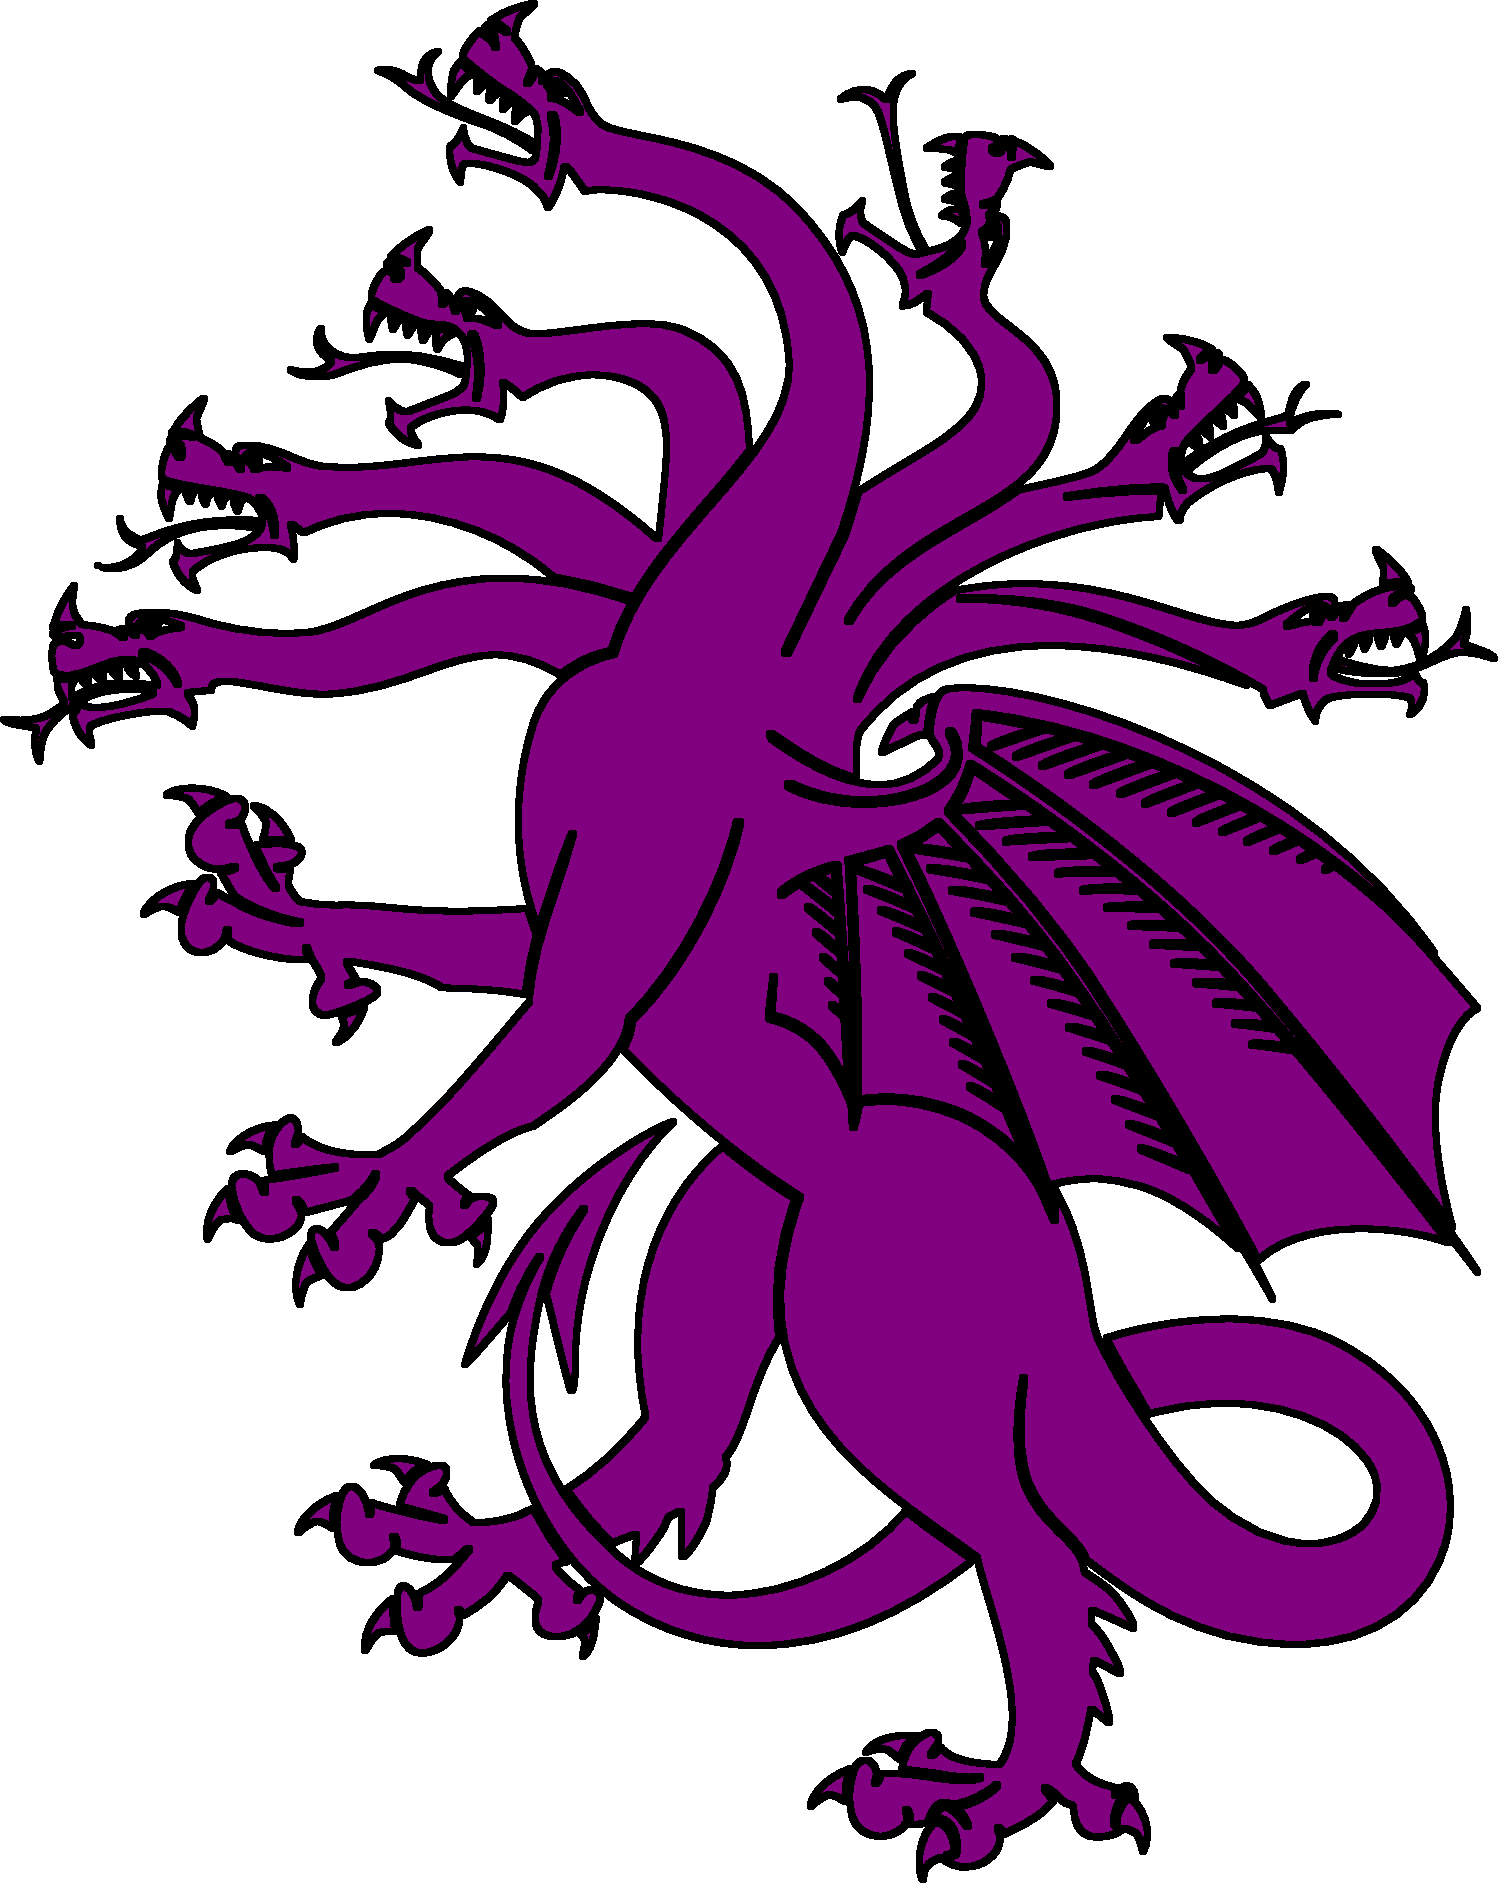
\includegraphics[scale=3.5]{Images/hydra.png}}; 
\end{scope}
}}

\tikzset{coa/.pic={
	\pic () at (0,0) {ribbon={#1}};
	\pic () at (0,8cm) {#1};
	\pic () at (0,8cm) {shield};
}}



\newlength{\cardwidth}
\newlength{\cardheight}
\newlength{\bleed}
\newlength{\horizspace}
\newlength{\vertspace}
\newlength{\vertdist}
\newlength{\horizdist}

\setlength{\cardwidth}{2.5in}
\setlength{\cardheight}{3.5in}
\setlength{\bleed}{0.0625in}
\setlength{\horizspace}{0.0625in}
\setlength{\horizdist}{\cardwidth + 2\bleed + \horizspace}
\setlength{\vertspace}{0.0625in}
\setlength{\vertdist}{\cardheight + 2\bleed + \vertspace}

\tikzset{guidecross/.pic={
	\draw (-\bleed,0) -- (\bleed,0);
	\draw (0, -\bleed) -- (0, \bleed);
}}

\tikzset{cutguide/.pic={
	\pic () at (-\cardwidth/2, \cardheight/2) {guidecross};
	\pic () at (\cardwidth/2, \cardheight/2) {guidecross};
	\pic () at (-\cardwidth/2, -\cardheight/2) {guidecross};
	\pic () at (\cardwidth/2, -\cardheight/2) {guidecross};
}}


\tikzset{cardbackpattern/.pic={
	\foreach \i in {-1.25, -1.0,...,1.25}
		\foreach \j in {-1.75, -1.5, ..., 1.75}
			\draw[very thick, #1] (\i,\j) circle (0.105);

	\foreach \i in {-1.375, -1.125, -0.875,...,1.125, 1.375}
		\foreach \j in {-1.875, -1.625, ..., 1.875}
			\draw[very thick, #1] (\i,\j) circle (0.105);
}}

\tikzset{cardbackprintable/.pic={
	\begin{scope}
	\clip (-\cardwidth/2 - \bleed, 0in) --%
	      (-\cardwidth/2 - \bleed, \cardheight/2 + \bleed) --%
	      (\cardwidth/2 + \bleed, \cardheight/2 + \bleed) --%
	      (\cardwidth/2 + \bleed, -\cardheight/2 - \bleed) --%
	      (-\cardwidth/2 - \bleed, -\cardheight/2 - \bleed) --%
	      cycle;
%	\path[fill=lightgray] (-\cardwidth/2 - \bleed, 0in) --%
%	      (-\cardwidth/2 - \bleed, \cardheight/2 + \bleed) --%
%	      (\cardwidth/2 + \bleed, \cardheight/2 + \bleed) --%
%	      (\cardwidth/2 + \bleed, -\cardheight/2 - \bleed) --%
%	      (-\cardwidth/2 - \bleed, -\cardheight/2 - \bleed) --%
%	      cycle;
	% Pattern for card back
	\pic () at (0,0) {cardbackpattern={#1}};
	\node[transform shape, rotate=-90, fill=White, fill opacity=1.0, text opacity=1.0, rounded corners=5mm] () at (0,0) {{\large\contour{White}{#1}}}; 	

	% Cutting guides for corners of the cards	
%	\pic () at (0,0) {cutguide};
\end{scope}
}}

\tikzset{charactercardfrontprintable/.pic={
	\begin{scope}
	\clip (-\cardwidth/2 - \bleed, 0in) --%
	      (-\cardwidth/2 - \bleed, \cardheight/2 + \bleed) --%
	      (\cardwidth/2 + \bleed, \cardheight/2 + \bleed) --%
	      (\cardwidth/2 + \bleed, -\cardheight/2 - \bleed) --%
	      (-\cardwidth/2 - \bleed, -\cardheight/2 - \bleed) --%
	      cycle;
	% Cutting guides for corners of the cards	
	\pic () at (0,0) {cutguide};
\end{scope}
}}

\setmainfont[Scale=3.0]{Cinzel}
\begin{document}
\setmainfont[Scale=1.0]{Cinzel}\phantom{a}\setmainfont[Scale=3.0]{Cinzel}
\begin{center}
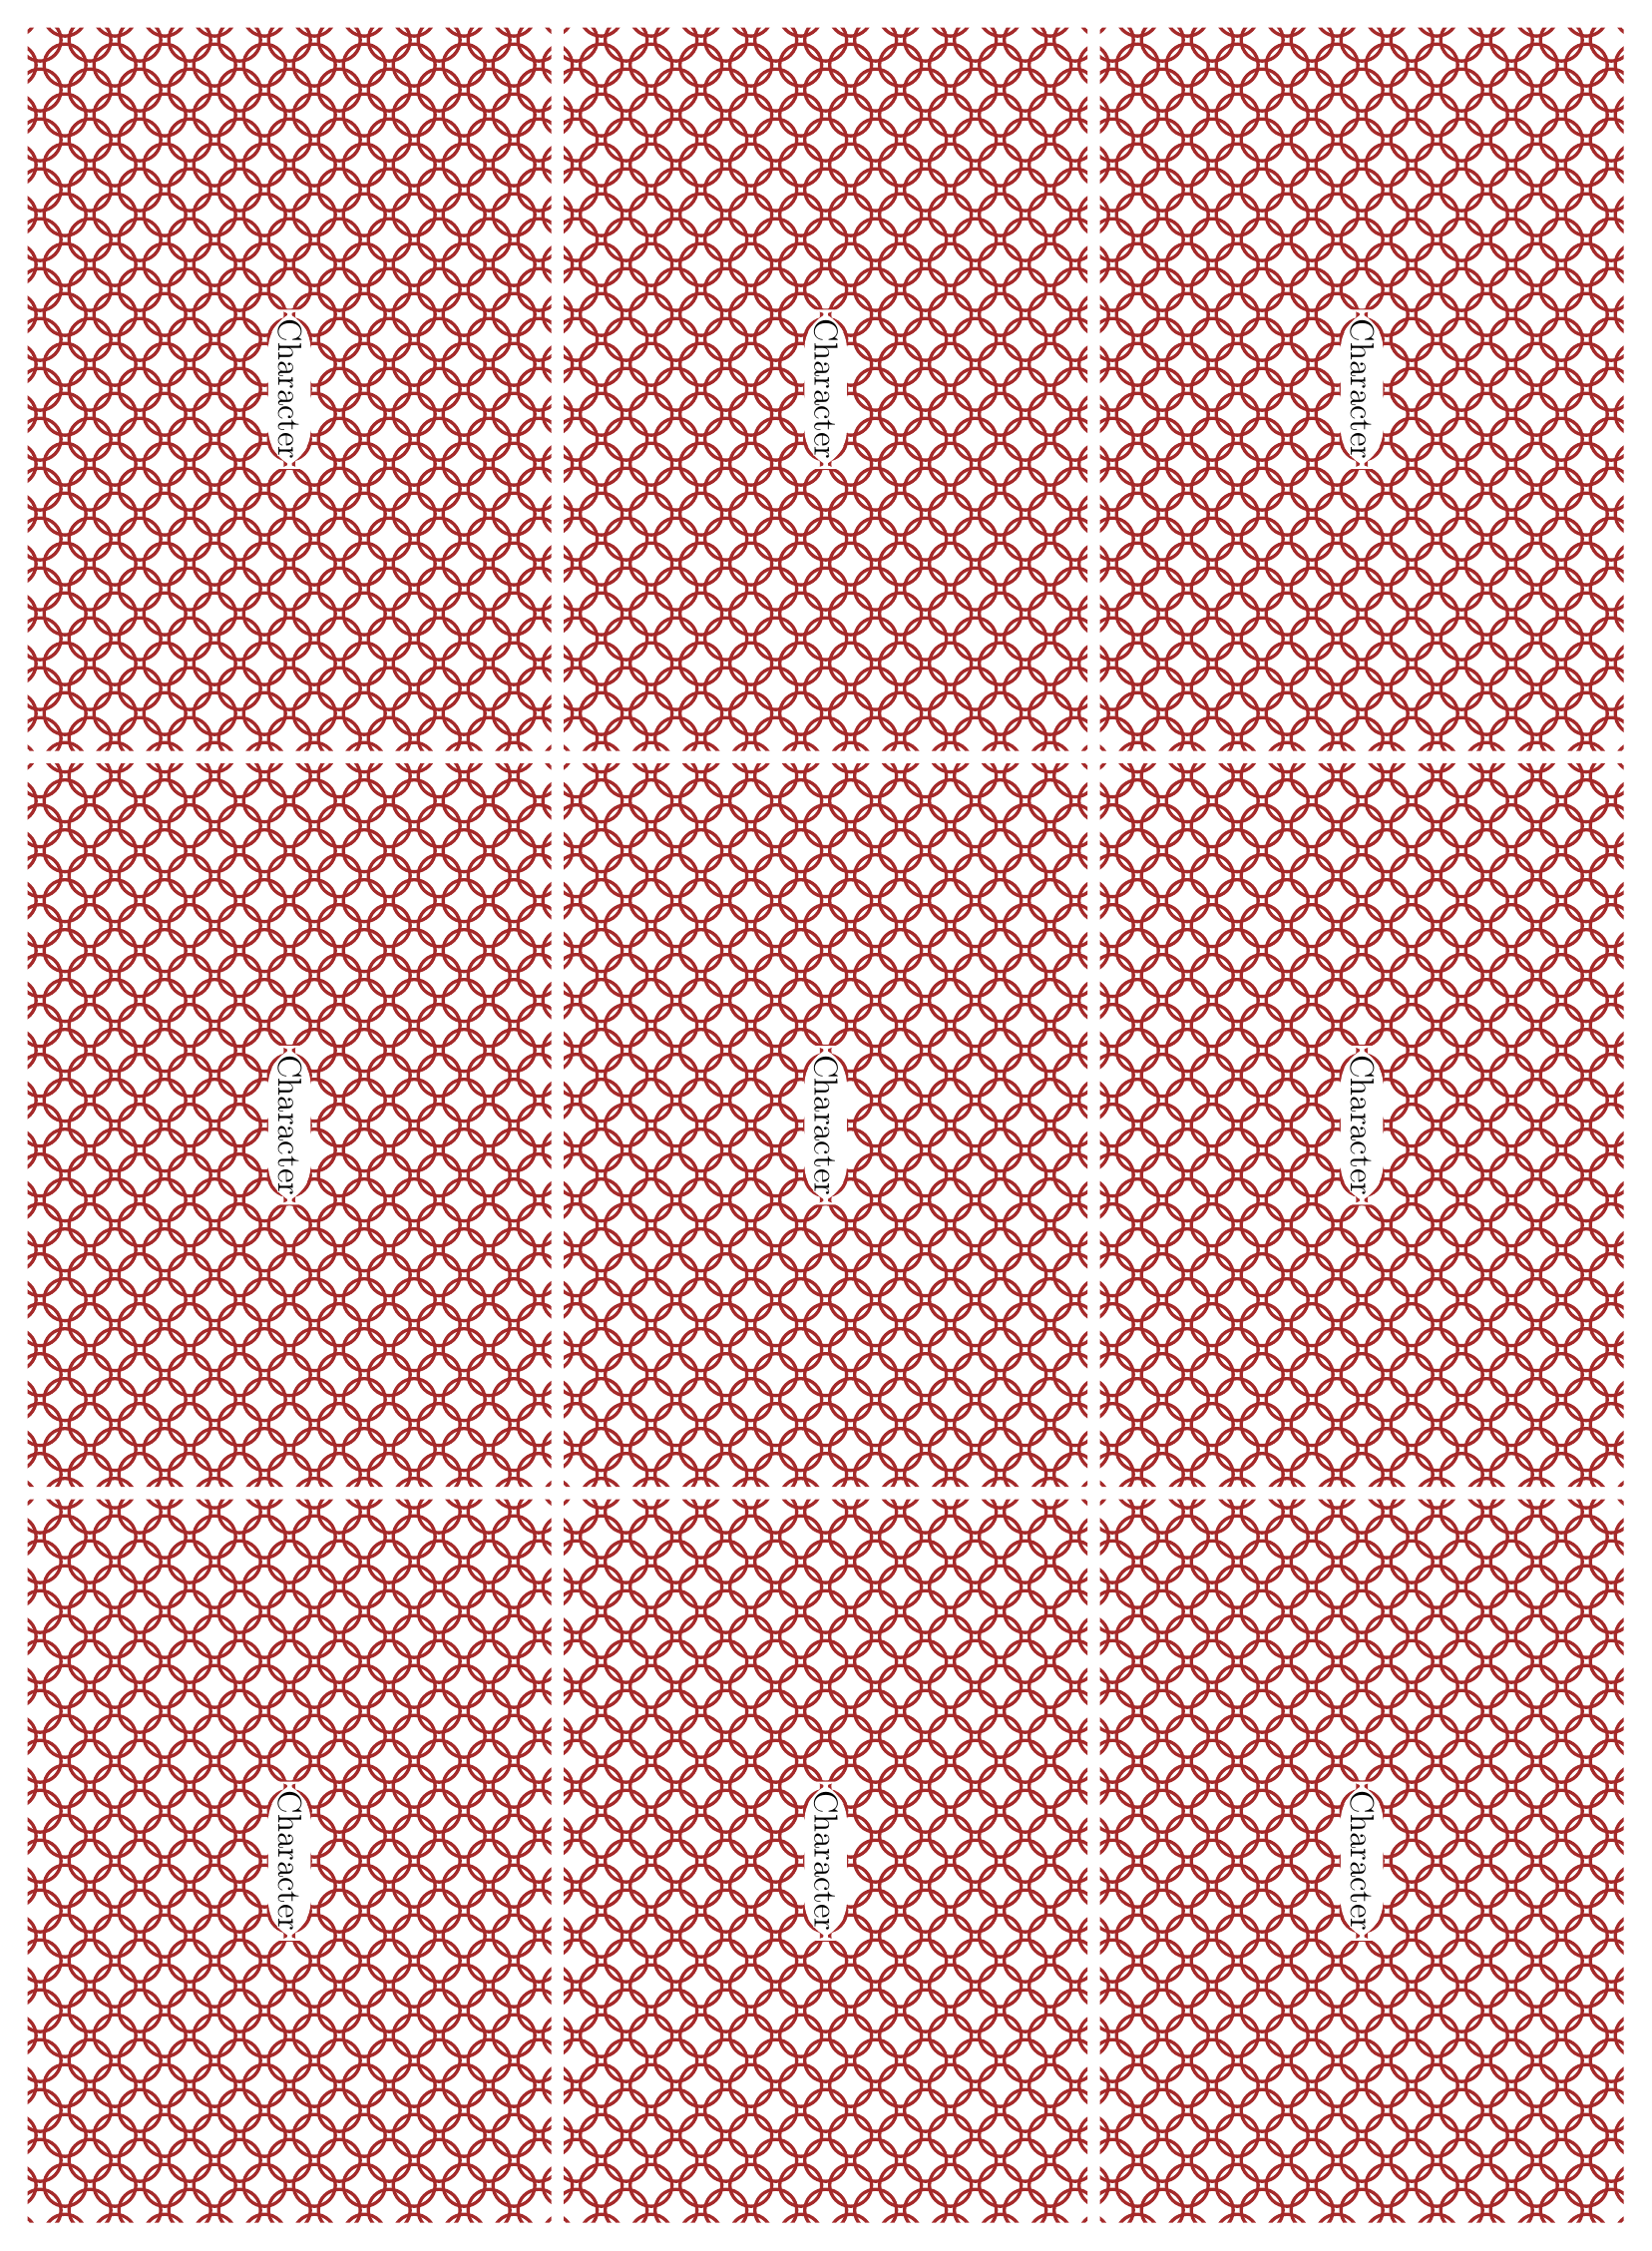
\begin{tikzpicture}[x=1in, y=1in]
\pic () at (0,0) {cardbackprintable={Character}};
\pic () at (\horizdist,0) {cardbackprintable={Character}};
\pic () at (2\horizdist,0) {cardbackprintable={Character}};

\pic () at (0,-\vertdist) {cardbackprintable={Character}};
\pic () at (\horizdist,-\vertdist) {cardbackprintable={Character}};
\pic () at (2\horizdist,-\vertdist) {cardbackprintable={Character}};

\pic () at (0,-2\vertdist) {cardbackprintable={Character}};
\pic () at (\horizdist,-2\vertdist) {cardbackprintable={Character}};
\pic () at (2\horizdist,-2\vertdist) {cardbackprintable={Character}};
\end{tikzpicture}	
\end{center}
\newpage
\setmainfont[Scale=1.0]{Cinzel}\phantom{a}\setmainfont[Scale=3.0]{Cinzel}
\begin{center}
\begin{tikzpicture}[x=1in, y=1in, transform shape]
\pic () at (0, 0) {cutguide};
\pic[rotate=90, scale=0.3, xshift=-4.5cm, yshift=-4.8cm] () at (0,0) {coa={Kida}};
\pic[rotate=90, scale=0.66, xshift=-3.6cm, yshift=0.4cm] () at (0,0) {seahorse};
\pic[xscale=-1, scale=0.66, rotate=-90, xshift=-3.6cm, yshift=0.4cm] () at (0,0) {seahorse}; 

\pic () at (\horizdist, 0) {cutguide};
\pic[rotate=90, scale=0.3, xshift=-4.5cm, yshift=-4.8cm] () at (\horizdist,0) {coa={Marus}};
\pic[rotate=90, scale=0.66, xshift=-3.6cm, yshift=0.4cm] () at (\horizdist,0) {seahorse};
\pic[xscale=-1, scale=0.66, rotate=-90, xshift=-3.6cm, yshift=0.4cm] () at (\horizdist,0) {seahorse}; 

\pic () at (2\horizdist, 0) {cutguide};
\pic[rotate=90, scale=0.3, xshift=-4.5cm, yshift=-4.8cm] () at (2\horizdist,0) {coa={Sorrell}};
\pic[rotate=90, scale=0.66, xshift=-3.6cm, yshift=0.4cm] () at (2\horizdist,0) {seahorse};
\pic[xscale=-1, scale=0.66, rotate=-90, xshift=-3.6cm, yshift=0.4cm] () at (2\horizdist,0) {seahorse}; 

\pic () at (0, -\vertdist) {cutguide};
\pic[rotate=90, scale=0.3, xshift=-4.5cm, yshift=-4.8cm] () at (0,-\vertdist) {coa={Kida}};
\pic[rotate=90, scale=0.66, xshift=3.3cm] () at (0, -\vertdist) {wolf};
\pic[xscale=-1, scale=0.66, rotate=-90, xshift=3.3cm] () at (0, -\vertdist) {wolf}; 

\pic () at (\horizdist, -\vertdist) {cutguide};
\pic[rotate=90, scale=0.3, xshift=-4.5cm, yshift=-4.8cm] () at (\horizdist,-\vertdist) {coa={Marus}};
\pic[rotate=90, scale=0.66, xshift=3.3cm] () at (\horizdist, -\vertdist) {wolf};
\pic[xscale=-1, scale=0.66, rotate=-90, xshift=3.3cm] () at (\horizdist, -\vertdist) {wolf}; 

\pic () at (2\horizdist, -\vertdist) {cutguide};
\pic[rotate=90, scale=0.3, xshift=-4.5cm, yshift=-4.8cm] () at (2\horizdist,-\vertdist) {coa={Sorrell}};
\pic[rotate=90, scale=0.66, xshift=3.3cm] () at (2\horizdist, -\vertdist) {wolf};
\pic[xscale=-1, scale=0.66, rotate=-90, xshift=3.3cm] () at (2\horizdist, -\vertdist) {wolf}; 

\pic () at (0, -2\vertdist) {cutguide};
\pic[rotate=90, yscale=1.0, xscale=1.25, yshift=0cm] () at (0, -2\vertdist) {eagle};
\pic[rotate=90, scale=0.3, xshift=-4.5cm, yshift=-5.65cm] () at (0,-2\vertdist) {coa={Kida}};

\pic () at (\horizdist, -2\vertdist) {cutguide};
\pic[rotate=90, yscale=1.0, xscale=1.25, yshift=0cm] () at (\horizdist, -2\vertdist) {eagle};
\pic[rotate=90, scale=0.3, xshift=-4.5cm, yshift=-5.65cm] () at (\horizdist,-2\vertdist) {coa={Marus}};

\pic () at (2\horizdist, -2\vertdist) {cutguide};
\pic[rotate=90, yscale=1.0, xscale=1.25, yshift=0cm] () at (2\horizdist, -2\vertdist) {eagle};
\pic[rotate=90, scale=0.3, xshift=-4.5cm, yshift=-5.65cm] () at (2\horizdist,-2\vertdist) {coa={Sorrell}};
\end{tikzpicture}	
\end{center}
\newpage
\setmainfont[Scale=1.0]{Cinzel}\phantom{a}\setmainfont[Scale=3.0]{Cinzel}
\begin{center}
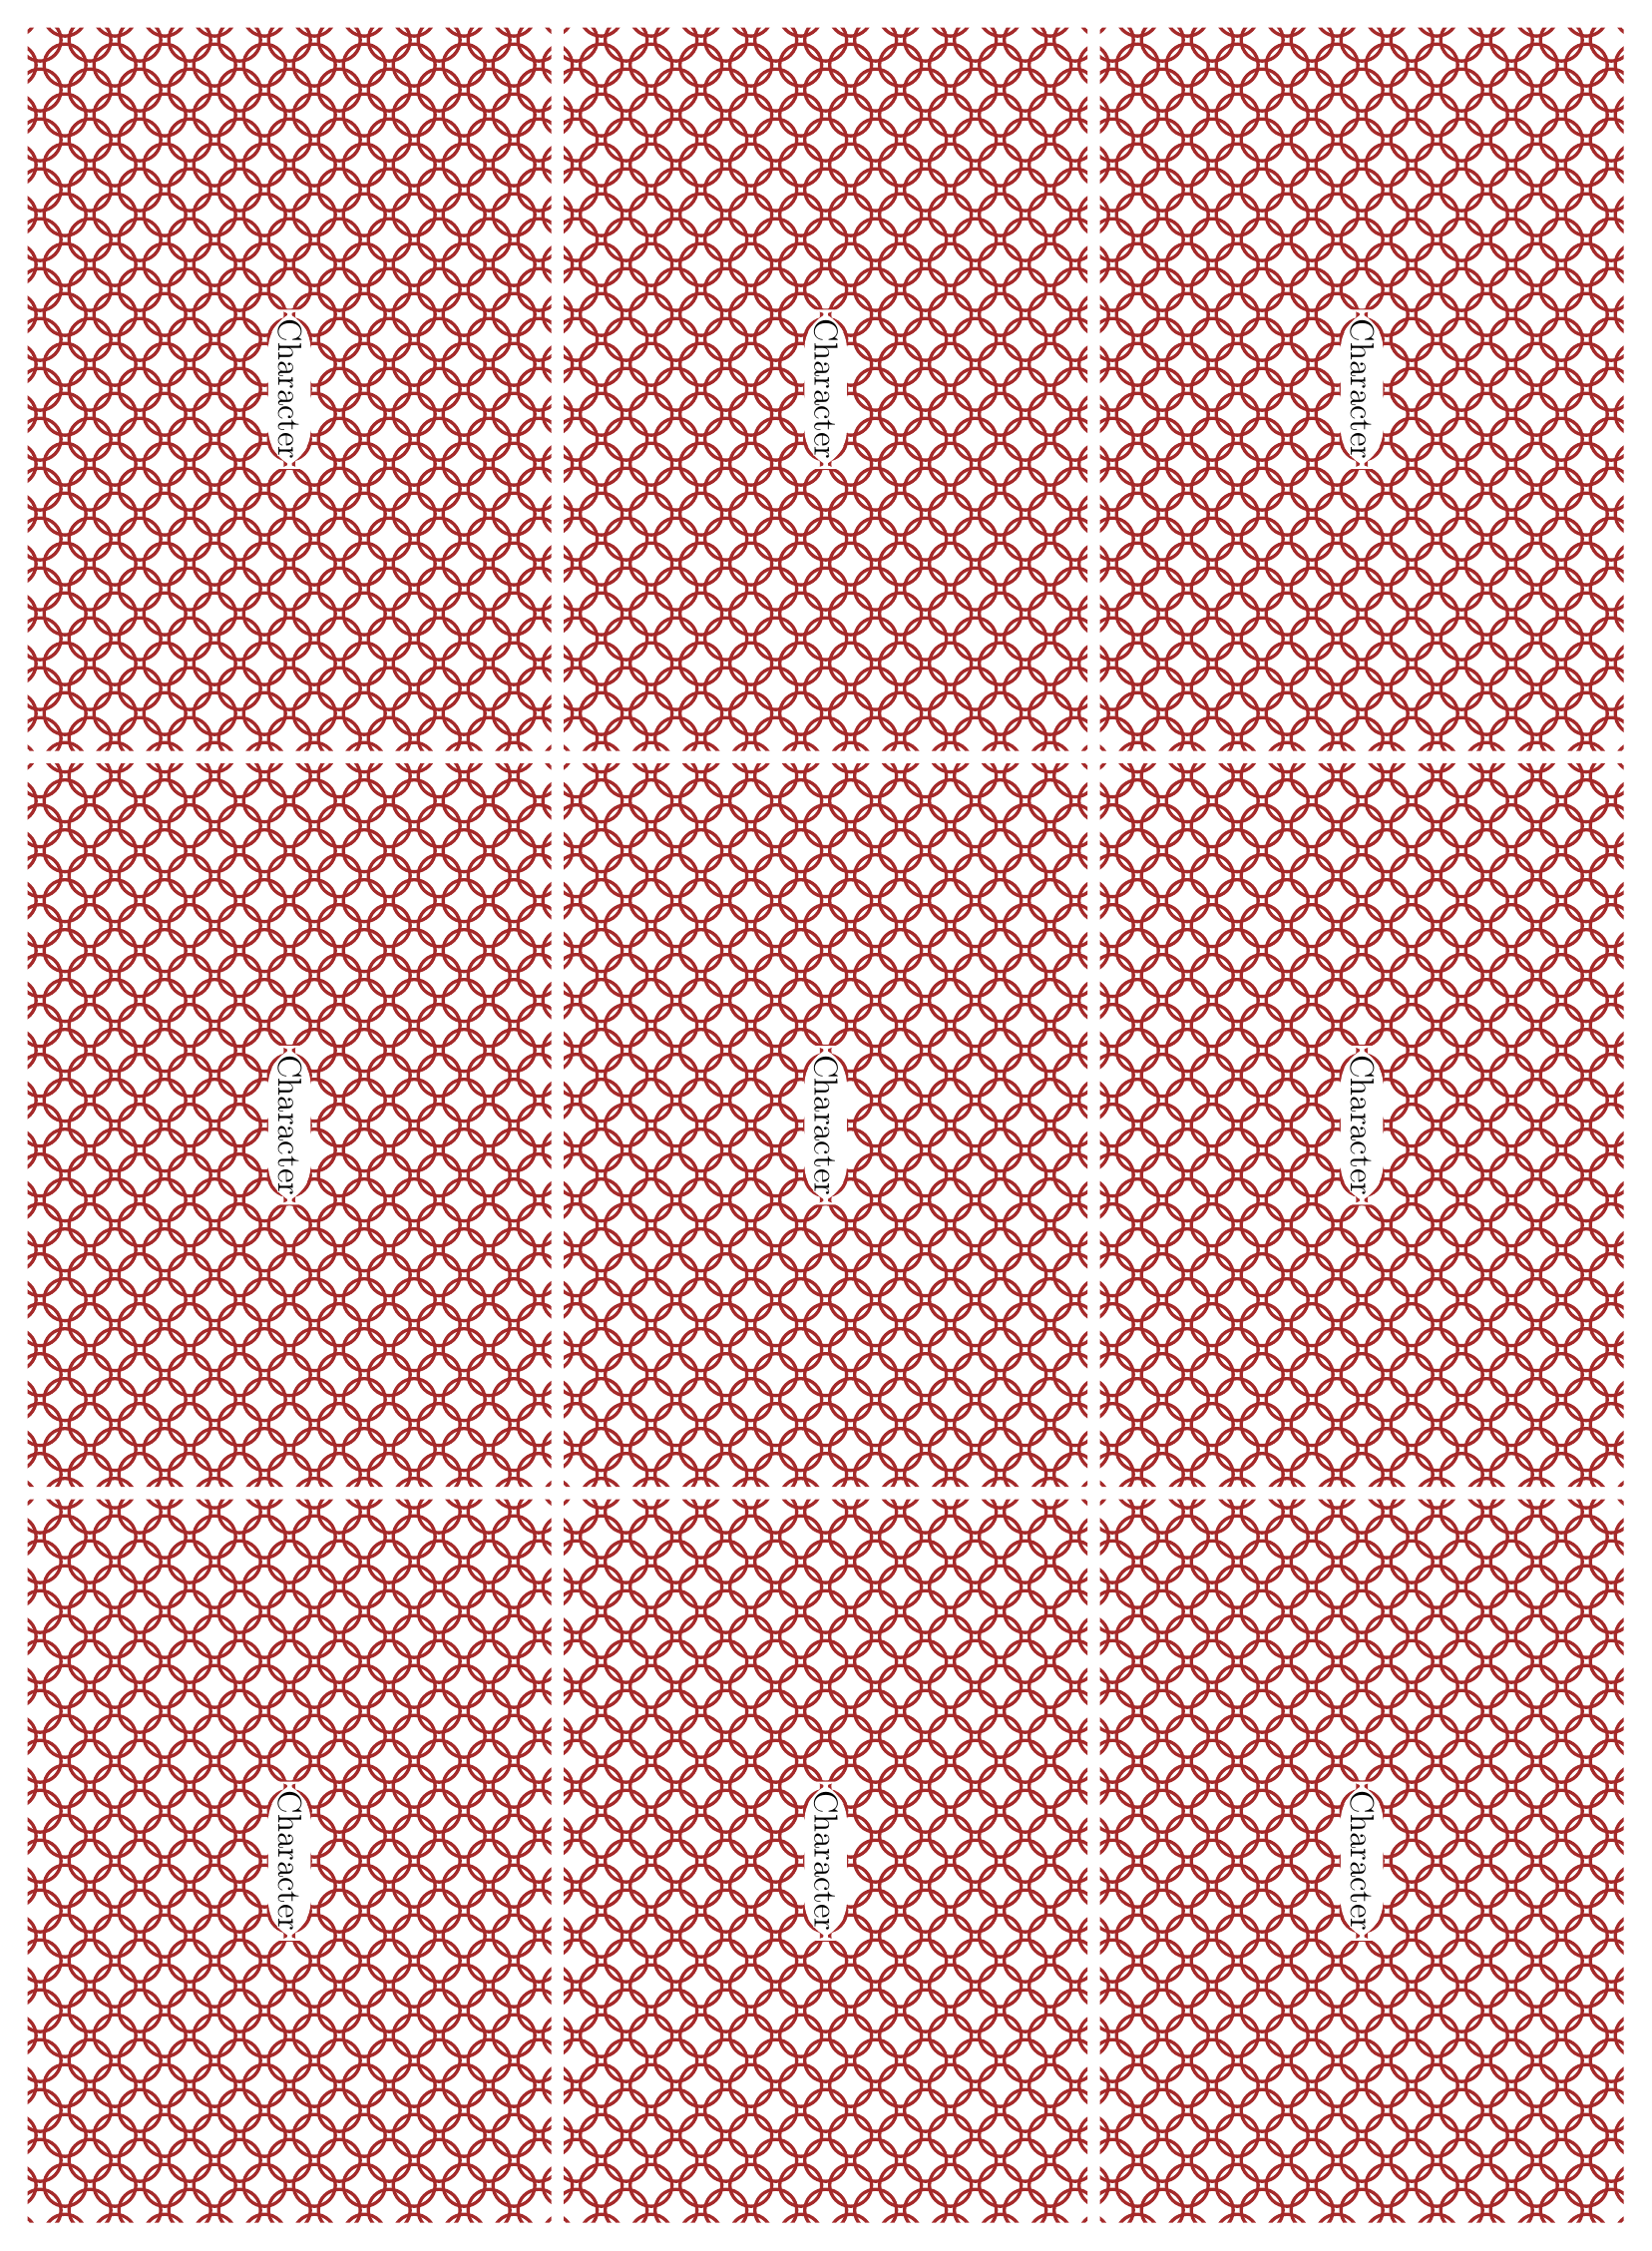
\begin{tikzpicture}[x=1in, y=1in]
\pic () at (0,0) {cardbackprintable={Character}};
\pic () at (\horizdist,0) {cardbackprintable={Character}};
\pic () at (2\horizdist,0) {cardbackprintable={Character}};

\pic () at (0,-\vertdist) {cardbackprintable={Character}};
\pic () at (\horizdist,-\vertdist) {cardbackprintable={Character}};
\pic () at (2\horizdist,-\vertdist) {cardbackprintable={Character}};

\pic () at (0,-2\vertdist) {cardbackprintable={Character}};
\pic () at (\horizdist,-2\vertdist) {cardbackprintable={Character}};
\pic () at (2\horizdist,-2\vertdist) {cardbackprintable={Character}};
\end{tikzpicture}	
\end{center}
\newpage
\setmainfont[Scale=1.0]{Cinzel}\phantom{a}\setmainfont[Scale=3.0]{Cinzel}
\begin{center}
\begin{tikzpicture}[x=1in, y=1in, transform shape]
\pic () at (0, 0) {cutguide};
\pic[rotate=90, scale=0.3, xshift=-4.5cm, yshift=-4.8cm] () at (0,0) {coa={Hydra}};
\pic[rotate=90, scale=0.66, xshift=-3.6cm, yshift=0.4cm] () at (0,0) {seahorse};
\pic[xscale=-1, scale=0.66, rotate=-90, xshift=-3.6cm, yshift=0.4cm] () at (0,0) {seahorse};

\pic () at (\horizdist, 0) {cutguide};
\pic[rotate=90, scale=0.3, xshift=-4.5cm, yshift=-4.8cm] () at (\horizdist, 0) {coa={Hydra}};
\pic[rotate=90, scale=0.66, xshift=3.3cm] () at (\horizdist, 0) {wolf};
\pic[xscale=-1, scale=0.66, rotate=-90, xshift=3.3cm] () at (\horizdist, 0) {wolf}; 

\pic () at (2\horizdist, 0) {cutguide};
\pic[rotate=90, yscale=1.0, xscale=1.25, yshift=0cm] () at (2\horizdist, 0) {eagle};
\pic[rotate=90, scale=0.3, xshift=-4.5cm, yshift=-5.65cm] () at (2\horizdist, 0) {coa={Hydra}};

\pic () at (\horizdist, -\vertdist) {cutguide};
\pic[rotate=90] () at (\horizdist, -\vertdist) {hydra};

\end{tikzpicture}	
\end{center}
\end{document}
